\textit{In order to do indoor flying there is a need of some sort of localization since GPS is not available indoor. Vision was decided based on what mostly others are using and some further advantages. Instead of making the vision, it is decided to use an existing tracker called MarkerLocator written by Henrik Midtiby. However the MarkerLocator lacks a proper quality measure so that is implemented. A few tests were made and the MarkerLocator with implemented quality measure is working quite well}


In order to do accurate flying indoor a localization system is needed. In the Related Work section, it can be seen vision with a camera mounted pointing down is used by others. Compared to use one or more cameras mounted on the drone, an advantage of using a camera mounted on the ceiling is that the camera will not be harmed if the drone crashes and that one camera can be used to detect several drones. However if the position is needed in more than 2D, more than one camera might be needed(depending on the algorithm used) but it still scales better than mounting one or more cameras on each drone. \\

Based on previous experience, the MarkerLocator written by Henrik Midtiby was chosen as indoor localization. Its using OpenCV\footnote{\url{http://opencv.org/}} and implemented in python. It works by detecting markers as shown in figure \ref{fig:markerlocator_marker}



\begin{figure}[H]
    \centering
    \begin{subfigure}[b]{0.2\textwidth}
        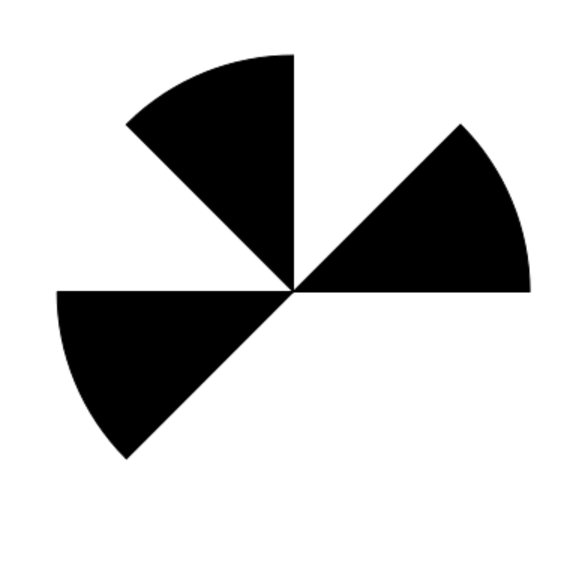
\includegraphics[width=\textwidth]{graphics/marker_order_4.pdf}
        \caption{Marker of order 4 used to get the 2D position of a drone}
        \label{fig:markerlocator_order_4}
    \end{subfigure}
    \quad %add desired spacing between images, e. g. ~, \quad, \qquad, \hfill etc. 
      %(or a blank line to force the subfigure onto a new line)
    \begin{subfigure}[b]{0.2\textwidth}
        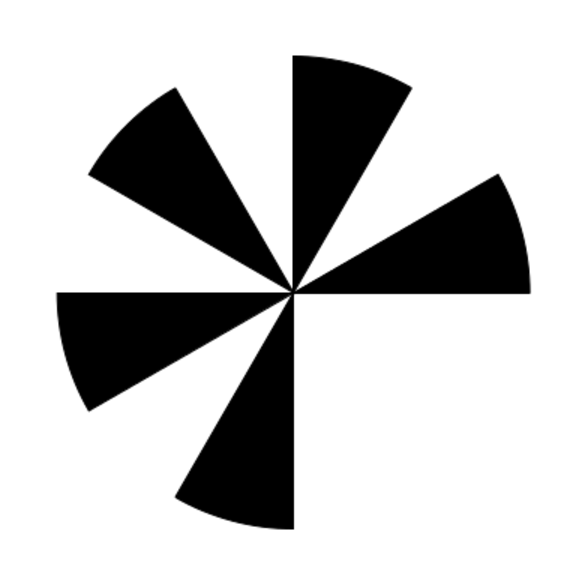
\includegraphics[width=\textwidth]{graphics/marker_order_6.pdf}
        \caption{Marker of order 6 used to get the 2D position of a drone}
        \label{fig:markerlocator_order_4}
    \end{subfigure}
    \caption{The markers have one arm less than the order of the marker for the MarkerLocator to detect the orientation of the marker}\label{fig:markerlocator_marker}
\end{figure}




The MarkerLocator works by making a convolution sum of a complex kernel on each frame obtained from the camera.
The location where if fits best is said to be the location of the marker in the frame.
How it works in detail is out the scope of this project.
The markers shown in figure \ref{fig:markerlocator_marker} is of different orders.
The order is equal to the number of black arms minus one since the missing arm is used to detect the orientation of the marker. 
Different orders can be used and thereby detect more than one marker in each frame. Unfortunately it can only get the 2D position and 1D orientation of the marker.
Since doing a convolution of the entire frame is relatively slow \footnote{Processing one fullHD frame takes approximately 0.38 sec. Measured with build in timer in the MarkerLocator}, the MarkerLocator has a mode called WindowMode.
It works by searching in only a small area around the last known position of the marker and thereby speeding up the progress\footnote{Approximately 0.0041 sec}. 

\begin{figure}[H]
    \center
    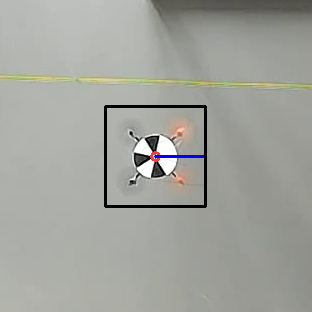
\includegraphics[width=0.4\textwidth]{graphics/markerlocator_window.png}
  	\caption{The MarkerLocator searches only for the marker around the last known position of the marker in a frame of 100*100px.}
    \label{markerlocator_windowmode}
\end{figure}
If the marker moves out of the window, the MarkerLocator is still looking in only that window.
Therefore it is important to have a quality measure that can be used to decide whenever a full convolution of the frame has to be done or if the marker has been found within the window. 

The MarkerLocator has a quality measure build-in used to tell how well the marker is detected. However it is not used in the MarkerLocator to tell if a full convolution has to be done. 
The quality measure implemented in the MarkerLocator is a hack \footnote{Said by Henrik Midtiby} and is known from previous applications that it is a bad measure of the right marker is detected.

In cooperation with Henrik Midtiby a few quality measures was developed. The overall idea was to compare the kernel used to do the convolution with the marker found in the frame.
Different algorithms where used to give a normalized value telling how similar the found marker is to the kernel. Figure \ref{fig:markerlocator_algorithms} shows the different solutions tried.\\

\begin{figure}[H]
    \centering
    \begin{subfigure}[b]{0.3\textwidth}
        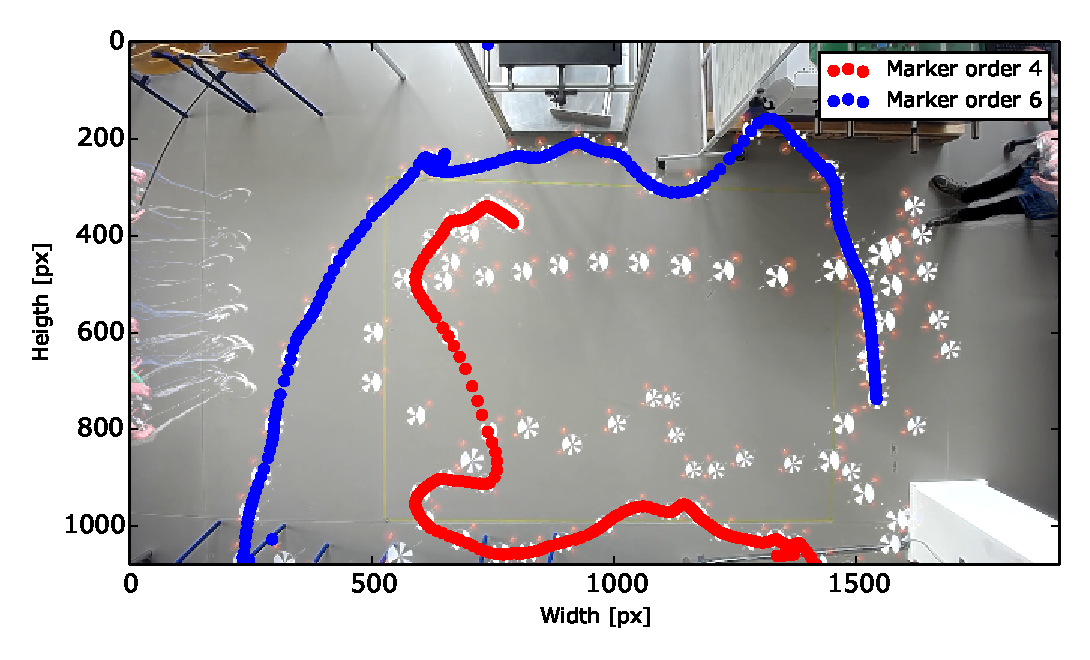
\includegraphics[width=\textwidth]{graphics/markerlocator_compare_raw.eps}
        \caption{Counting pixel match suffers from being unable to find the markers if lost}
        \label{fig:markerlocator_algorihm_native}
    \end{subfigure}
    ~ %add desired spacing between images, e. g. ~, \quad, \qquad, \hfill etc. 
      %(or a blank line to force the subfigure onto a new line)
    \begin{subfigure}[b]{0.3\textwidth}
        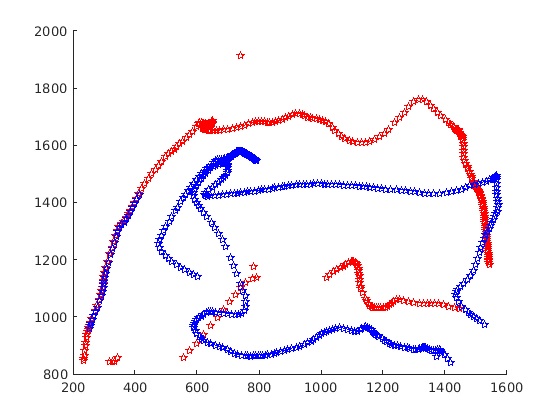
\includegraphics[width=\textwidth]{graphics/markerlocator_ssim.png}
        \caption{SSIM suffers from false positives and a few false negative}
        \label{fig:markerlocator_algorithm_ssim}
    \end{subfigure}
    ~
    \begin{subfigure}[b]{0.3\textwidth}
        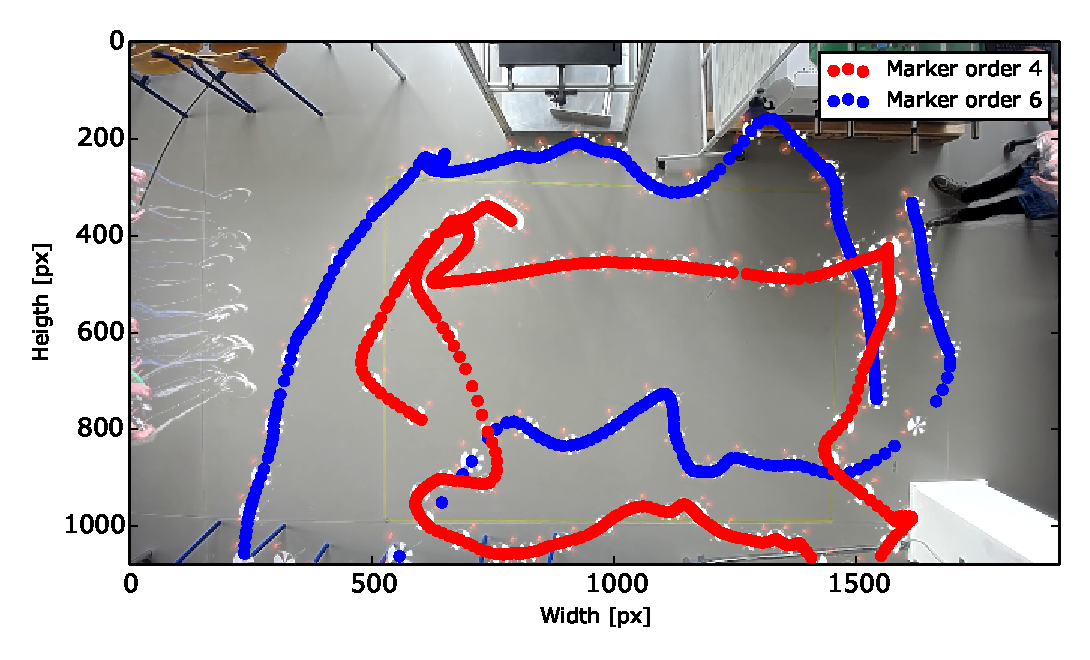
\includegraphics[width=\textwidth]{graphics/markerlocator_match_order.eps}
        \caption{Developed algorithm has no false negative of positive and is able to find the markers if lost}
        \label{fig:markerlocator_algorithm_order_match}
    \end{subfigure}
    \caption{Different approaches to get a quality measure explaining how well the right marker is found.}\label{fig:markerlocator_algorithms}
\end{figure}

Figure \ref{fig:markerlocator_algorihm_native} is a native approach of comparing all pixels in the kernel with the pixels in the found marker. A counter is incremented upon each match and at the end divided by the number of pixels compared in to normalize. A threshold determines weather a marker is found and the next scan should be done in the window of if a full scan is required. The best result is obtained using a threshold of 0.4. If the threshold were lowered false positives started to occur. \\

Figure \ref{fig:markerlocator_algorithm_ssim} uses an algorithm developed to compare similarities in images. 
The details of this algorithm is out of scope the details of this project. The implementation in scipy-image\footnote{\url{http://scikit-image.org/}} was used.
It can seen it performs better than the native approach but a lot of false positive and a few false negative exists. It also suffers from not detecting the markers compared to the native approach. A threshold of 0.3 were used. If the threshold were increased, it would detect less markers. \\

Figure \ref{fig:markerlocator_algorithm_order_match} shows a simple algorithm the author came up with.
If the MarkerLocator is looking for a marker of order 4 and it has detected a marker and its orientation, the algorithm calculates where the location of the arms. It then checks a pixel in each arm and increments a counter if the pixel is black. When it has checked all the arms it compares the counter with the order the MarkerLocator is looking for and returns if they match or not. 
This method does not provide a scalar as output but a binary and thereby has no threshold. However in order to detect if a pixel is black or not, a threshold has been used. The threshold was set to 100 which has shown good results doing tests and flight. \\

During development of quality measures it was noted that if the MarkerLocator does a full search because it cannot find a marker with order 4, it slows down the detection of the marker of order 6. This is because the MarkerLocator is implemented in one process without threading. However this has been solved by splitting up the MarkerLocator in different processes so they run independently of each other. More about this in section  \ref{sec:system_architecture_indoor} \\

\textbf{Perspective correction} \\
In order to use centimeters as measure of the position of the markers and to correct if the camera is not pointing directly down, the build-in perspective correction in the MarkerLocator were used.
It works by using homography\cite{janeriksolem2012} to make the transformation from pixels to some chosen unit which in this case is centimeters.
\begin{wrapfigure}{r}{0.4\textwidth}
  \vspace{-20pt}
  \begin{center}
    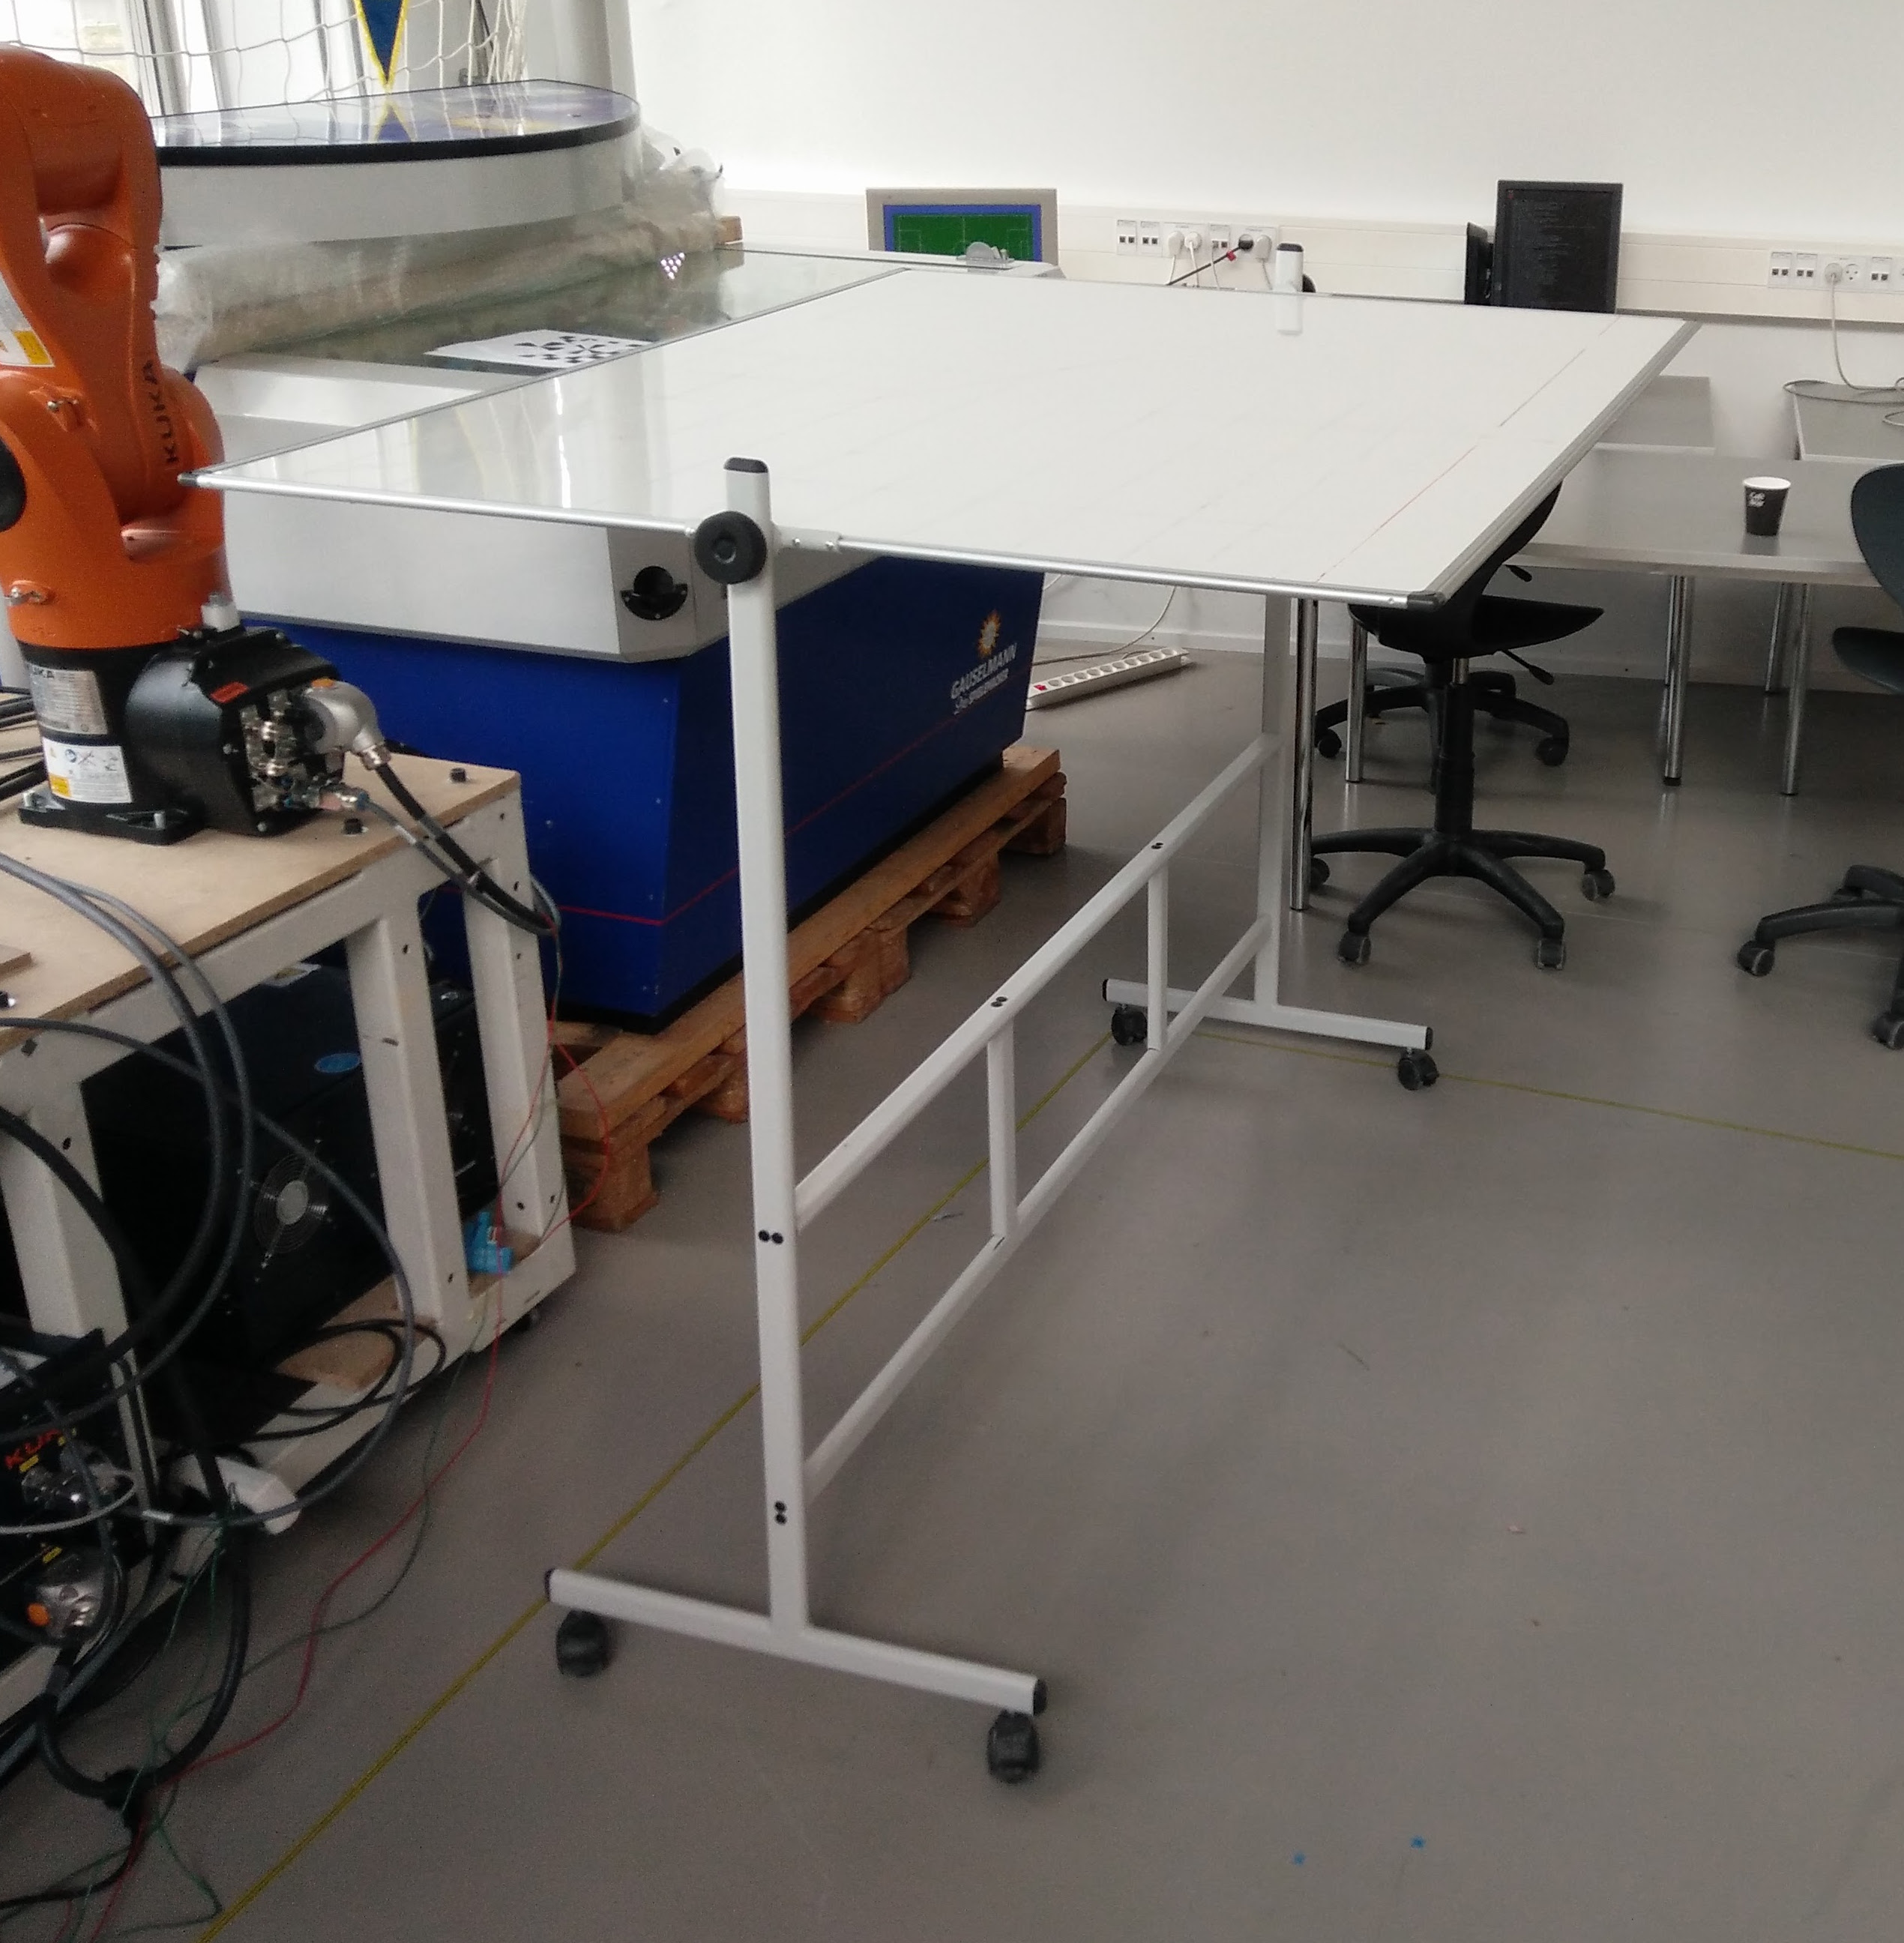
\includegraphics[width=0.48\textwidth]{graphics/whiteboard_tilted.jpg}
  \end{center}
  \vspace{-20pt}
  \caption{Setup used to make 4 points in the flight-height. The four corners of the whiteboard was used and then found in the image. } \label{fig:whiteboard_setup}
  \vspace{-10pt}
\end{wrapfigure}

By creating four markers with known distance to each other at the expected flight height \footnote{Since only 2D positioning is available, a plane where the drone is expected to fly is decided} and find these markers in the frame, it is possible for the perspective corrector to make the transformation.
Figure \ref{fig:whiteboard_setup} shows the setup used. A picture was taken from the ceiling-camera and the four black corners of the whiteboard could be found in the frame. The distance between the black corners in centimeters and the distance in px is given as input to the perspective correcter. The locations of markers is then transformed into the plane made by the whiteboard. Depending on where the whiteboard is placed in the frame origin can be placed. The placement of the coordinate system can be seen in section \ref{sec:coordinate_system}\\


A test was conducted to get the accuracy of the MarkerLocator. Two markers with order 4 and 6 was placed at the expected flight-height and the distance between the two markers was calculated using Pythagoras.\\
This was done with distance 60 centimeters measured using a ruler. 
The real distance measured by a ruler was 60 cm and and the MarkerLocator gave 

Another test was conducted in order to see how stable the MarkerLocator is. 547 position detections was done while the marker was placed steady at the flight height. It shows a mean position in x of -8.1487 with variance of 0, y position with mean -39.5046 and variance 0. \\

Some of this inaccuracy is caused by measuring error and placing of the whiteboard. If higher accuracy is needed this should be done again more carefully.

It can be concluded that using the MarkerLocator with the improved order detection it is possible to detect two drones without having any false positive/negative. By making a test of the distance between two markers there is an error of 0.81 cm. The MarkerLocator seems stable with a variance of zero. 

